\documentclass[tikz, border=10pt]{standalone}
\usetikzlibrary{automata, positioning, arrows}
\usepackage{amsmath}

\begin{document}

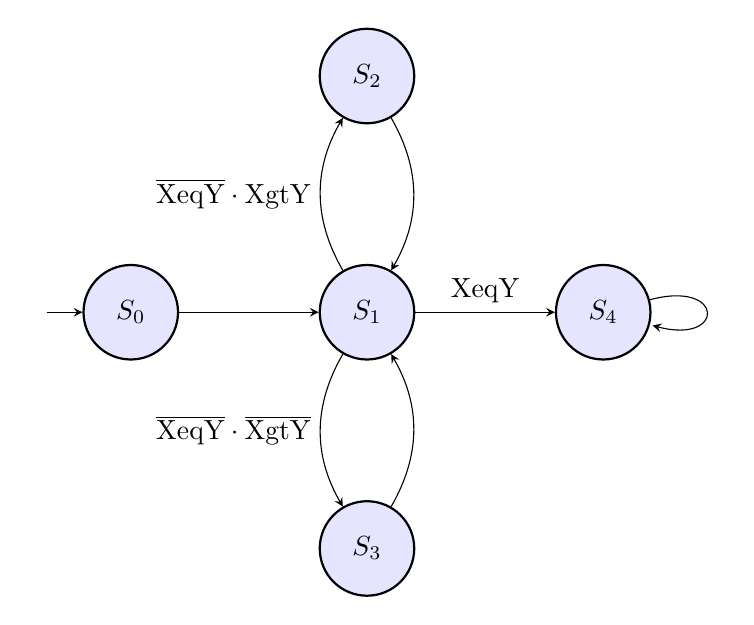
\begin{tikzpicture}[
    ->, >=stealth, auto, node distance=3cm,
    every state/.style={thick, fill=blue!10, minimum size=1.2cm},
    initial text=$ $
]

    \node[state, initial] (S0) {$S_0$};
    \node[state, right of=S0] (S1) {$S_1$};
    \node[state, above of=S1] (S2) {$S_2$};
    \node[state, below of=S1] (S3) {$S_3$};
    \node[state, right of=S1] (S4) {$S_4$};

    \path   (S0) edge node {} (S1)
            (S1) edge node {XeqY} (S4)
            (S1) edge [bend left] node [left] {$\overline{\text{XeqY}} \cdot \text{XgtY}$} (S2)
            (S1) edge [bend right] node [left] {$\overline{\text{XeqY}} \cdot \overline{\text{XgtY}}$} (S3)
            (S2) edge [bend left] node {} (S1)
            (S3) edge [bend right] node {} (S1)
            (S4) edge [loop right] node {} (S4);

\end{tikzpicture}

\end{document}
